% ============================================================================ FRAMEWORK
\section{Framework}\label{sec:framework}

\begin{figure*}[!t]
\centering
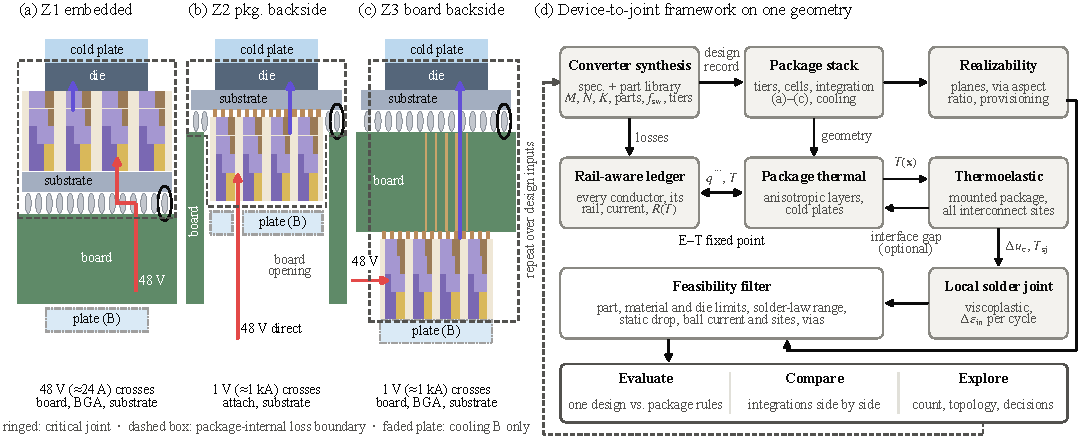
\includegraphics[width=\textwidth]{fig1_concept_framework.pdf}
\caption{(a)--(c) Three integrations of the same regulator cells: embedded between the
substrate and the die (Z1), attached to the substrate backside inside a board opening (Z2), and
mounted on the board backside (Z3). The integration decides which rail crosses the substrate and
the board, at what current, and which solder joints carry the deformation (ringed: critical
joint). The 48-V feed of Z2 and Z3 starts outside the package-internal loss boundary (dashed
box). Schematic; to-scale sections in Fig.~\ref{fig:sections}. (d) The framework: what each
stage hands to the next on one geometry. Double arrow: the bidirectional electrothermal (E--T)
fixed point; single arrows: one-way transfers; dotted: the optional mechanical-to-thermal
feedback through the top thermal interface; dashed: the exploration loop over the design
inputs.}
\label{fig:concept}
\end{figure*}

The framework is a chain of models that share one geometry (Fig.~\ref{fig:concept}). Its inputs
are a system specification---load power and voltage, input rail, die footprint, a target
regulator current density and an allowable ripple---a component library of power devices,
inductors and capacitors, an integration architecture and a cooling solution, given as the
boundaries it imposes (a film coefficient and coolant inlet temperature on each cooled face, or
a coolant model that computes them). Its outputs are a synthesized regulator, an explicit
package stack, a conductor-level loss ledger, converged temperature, deformation and
joint-response fields, a feasibility verdict, and the uncertainty of each output.

\emph{Converter synthesis} enumerates hybrid switched-capacitor--buck topologies and selects
devices, passives and switching frequency for the specified regulator count by exhaustive
search over a discrete library (Section~\ref{sec:dse}). \emph{Stack construction} turns the
selected components into tiers inside each cell footprint, adds the interlayer
redistribution, places the cells in the chosen integration and builds the substrate,
interconnect fields, board, ball field and cooling boundaries around them. The \emph{rail-aware
ledger} assigns to every conductor the rail it carries and that rail's current, and evaluates
its resistance from geometry and temperature. The \emph{package thermal model} receives the
ledger as a heat map deposited where each loss is generated and returns temperatures, which
update every temperature-dependent resistance. The converged field drives a
\emph{thermoelastic package model} of the mounted assembly, which searches every legal
solder-joint site for the largest relative displacement, and a \emph{local viscoplastic
submodel} of the critical joint and its alternatives, which returns their inelastic response per
thermal cycle. The \emph{feasibility} stage checks the result against the ratings of the
selected components and the rules of the package: power-device junction temperature, capacitor,
inductor and package-material limits, the validity range of the solder law, via aspect ratio,
pitch and landing area, and ball and attach provisioning.

\emph{One geometry} has a precise meaning here. Every stage derives its domain from one stack
description: the ledger takes conductor lengths, cross sections and counts from it, and the two
finite-element models discretize it into one mesh. Each ledger term names the layer and the
cell footprints that produce it, and these map to element sets of that mesh; the heat deposited
in them equals the ledger total to $10^{-6}$, and the temperature returned to a term is the mean
over the nodes of the same set. The mechanics reads the converged nodal field on the same mesh,
and the local submodel reads the displacement and temperature of a ball site of the same
lattice the ledger provisions. Three different kinds of interaction follow, and the framework
keeps them apart (Fig.~\ref{fig:concept}d). \emph{Coupled solution}: loss and temperature are
solved together, by fixed-point iteration, because each changes the other at first order.
\emph{One-way transfer}: the converged temperature field loads the mechanics, and the critical
joint's displacement and temperature drive the local submodel; nothing is returned.
\emph{Neglected feedback}: the mechanical state does not update the electrical or thermal model
in production. The thermal strain of a copper conductor, $\alpha_{\mathrm{Cu}}\Delta T\approx
0.15$\,\%, changes its resistance two orders of magnitude less than the 20--35\,\% change of
resistivity inside the fixed point, so the electrical feedback is negligible. The thermal
feedback is not always negligible: when a flat cold plate meets a warped die, the thermal
interface thickens where the die falls away. The framework closes this loop as an option, and
Section~\ref{sec:compare} quantifies it. Contact degradation, delamination, intermetallic
growth and damage are outside the intact-package scope.

\begin{figure}[!t]
\centering
\fbox{\begin{minipage}{0.95\columnwidth}\footnotesize
\textbf{Input:} specification, library, integration, cooling boundaries.\\[2pt]
\textbf{1} \;Synthesize the regulator: exhaustive search over topologies, devices, passives
and $f_{\mathrm{sw}}$ under rating, ripple and area constraints (Section~\ref{sec:dse}).\\
\textbf{2} \;Build the stack and the mesh; check via aspect ratio, pitch, landing and
provisioning (Section~\ref{sec:realizability}).\\
\textbf{3} \;Set the region temperatures $T^{0}$.\\
\textbf{4} \;\textbf{repeat}: ledger $L(T^{k})$; deposit $L$ by region (deposit = ledger total);
solve the thermal field with the cooling boundaries; $T^{k+1}$ = region means;\\
\hspace*{1.2em}\textbf{until} $\max|T^{k+1}-T^{k}| < 0.25$~K and $|\Delta P|/P < 10^{-3}$.\\
\textbf{5} \;Solve the thermoelastic package on the converged field; evaluate $\Delta u$ at
every legal ball site.\\
\textbf{6} \;\emph{Optional}: update the interface thickness from the solved warpage and
return to 4, until the warpage changes by less than 1\,\%.\\
\textbf{7} \;Solve the local submodel at the site of largest $\Delta u$ and at the competing
sites (largest $T_{\mathrm{j}}$, corners, the Pareto set in $\Delta u$ and $T_{\mathrm{j}}$);
report the largest response.\\
\textbf{8} \;Check feasibility: junction, component and material temperatures against their
ratings, joint temperature against the solder law, interconnect rules.\\[2pt]
\textbf{Output:} loss by conductor and component, temperatures, warpage, $\du$,
$\deps$, verdicts, and the uncertainty of each.
\end{minipage}}
\caption{One evaluation of the framework. Steps 1 and 2 are analytical (seconds); step 4 is
the only coupled solution; steps 5 and 7 are one-way transfers.}
\label{fig:algorithm}
\end{figure}

Because every stage reads and writes the same geometry, the framework can be used in three ways
(Fig.~\ref{fig:algorithm}). To \emph{evaluate} a design, the chain is run once and every output
is checked against the ratings and rules of the feasibility stage. To \emph{compare}
integration architectures, the same synthesized regulator is placed in each candidate under the
same cooling boundaries; every output is reported side by side, inside explicitly declared loss
boundaries, and candidates that fail a rating are filtered out before any ranking. To
\emph{explore} the design space, converter synthesis is repeated over regulator count and
topology as an electrical screen, the strongest candidates are carried through the coupled
chain, and every package input without a single defensible value is varied on the production
mesh, so that each ranking is reported together with the decisions that can reverse it.
